\section{Organization}

\newcommand{\bluefat}[1]{\textcolor{faublue}{\textbf{#1}}}

\begin{frame}[t]{Pattern Recognition}
    \begin{block}{Consisting of}
        \begin{itemize}
            \item 3.75 ECTS Lecture $\Rightarrow$ 4 short videos per week (15 minutes each)
            \item 1.25 ECTS Exercises $\Rightarrow$ 1.5h exercise session per week
        \end{itemize}
    \end{block}

    \vspace{0.3cm}
    \begin{itemize}
        \setlength\itemsep{0.3cm}
        \item \bluefat{Lecture:} principles of classification and regression
        \item \bluefat{Exercises:}
              \vspace{0.3cm}
              \begin{itemize}
                  \setlength\itemsep{0.2cm}
                  \item \bluefat{Theory:} broadening of mathematical foundations
                  \item \bluefat{Programming:} implementation of learned classifiers
                  \item Theory and programming will switch every week
              \end{itemize}
    \end{itemize}

\end{frame}

\begin{frame}[t]{Lecture}

    Monday, Tuesday, Wednesday, Thursday

    \vspace{0.3cm}
    \begin{itemize}
        \setlength\itemsep{0.3cm}
        \item Four 15min videos will be scheduled every week
        \item Recordings only
        \item \href{https://www.video.uni-erlangen.de/course/id/1579}{Recordings on \bluefat{fau.tv}}
        \item \href{https://www.youtube.com/watch?v=8cZ-ljrSaEw&list=PLpOGQvPCDQzsWvT_bqmexrJ359RTQQuMO}{Recordings with \bluefat{YouTube} reminders}
        \item Questions? $\Rightarrow$ Exercise sessions, MS Teams, StudOn
    \end{itemize}
    \vspace{0.3cm}
    \begin{block}{Contents}
        \begin{itemize}
            \setlength\itemsep{0.1cm}
            \item Introduction and principles of pattern recognition
            \item Classification and regression algorithms
            \item Foundations of estimation and optimization theory
        \end{itemize}
    \end{block}
\end{frame}

\begin{frame}[t]{Theory Exercises}

    Wednesday 4:15pm \bluefat{or} Friday 12:15pm

    \vspace{0.3cm}
    \begin{itemize}
        \setlength\itemsep{0.3cm}
        \item Theoretical and programming exercises switch every other week
        \item Both sessions offer same content $\Rightarrow$ choose one
        \item \href{https://fau.zoom.us/j/95317133405?pwd=c3dpSUc1WkNHU3haZHg5NERyNXAxUT09}{\bluefat{Zoom on Wednesday} (Password 634093)}
        \item \href{https://fau.zoom.us/j/92488417095?pwd=UzJIdE55eHpGdlBRU2pqZk51eGIydz09}{\bluefat{Zoom on Friday} (Password 202221)}
        \item Recordings on \href{https://www.video.uni-erlangen.de/course/id/1578}{\bluefat{fau.tv}}
    \end{itemize}

    \vspace{0.3cm}
    \begin{block}{Advise}
        \begin{itemize}
            \setlength\itemsep{0.3cm}
            \item We will solve exercise sheets with problems from the lecture
            \item Try to solve them yourself as a preparation!
        \end{itemize}
    \end{block}
\end{frame}

\begin{frame}[t]{Programming Exercises}

    Wednesday 4:15pm \bluefat{or} Friday 12:15pm

    \vspace{0.3cm}
    \begin{itemize}
        \setlength\itemsep{0.1cm}
        \item \href{https://teams.microsoft.com/l/team/19\%3ad1b741fa9b234318b83d6a50d3f22e0f\%40thread.tacv2/conversations?groupId=164543b9-54c7-4cdb-949a-37b423cd4158&tenantId=b2efcef3-8496-40b8-9de8-f135982f3461}{\bluefat{Join this class}} with access code j8c44n0 (\href{https://www.anleitungen.rrze.fau.de/medien/ms-teams/}{\bluefat{Activate MS Teams first}})
        \item Five programming problems in Python
        \item Implementation of classifiers with graphical visualization
        \item No need to submit solutions
        \item Solutions will be provided after period to solve the problems

    \end{itemize}

    \vspace{0.3cm}
    \begin{block}{Advise}
        \begin{itemize}
            \setlength\itemsep{0.3cm}
            \item Try to solve them yourself!
            \item Make sure you know about the basic usage of Numpy (e.g. by doing a \href{https://sebastianraschka.com/blog/2020/numpy-intro.html}{\bluefat{online tutorial}})
            \item Rely on team work and attendance of the exercises when you need assistance.
        \end{itemize}
    \end{block}
\end{frame}

\begin{frame}[t]{Exam}

    \begin{itemize}
        \setlength\itemsep{0.3cm}
        \item 60 minutes written exam
        \item 5 topics for the \st{presentation}
            \vspace{0.3cm}
            \begin{itemize}
                \setlength\itemsep{0.3cm}
                \item 3 topics from lecture
                \item 1 topic from theory exercise
                \item 1 topic from programming exercise
            \end{itemize}
        \item There will be a mock exam in January
    \end{itemize}

    \vspace{0.3cm}
    \begin{center}
        \alert{Due to unexpected high demand for the course (over 500 students!) we have to move to a written format!
        We will try to find a solution for students who cannot attend an in-person exam.}
    \end{center}
    
\end{frame}

\begin{frame}[t]{University Code of Conduct}

    \begin{itemize}
        \setlength\itemsep{0.3cm}
        \item[$\Rightarrow$] We are not responsible for your studies, you are!
        \item[$\Rightarrow$] No obligatory submissions or evaluation during semester
        \item[$\Rightarrow$] Choose the best way for you to learn and prepare for exam:
              \vspace{0.3cm}
              \begin{itemize}
                  \setlength\itemsep{0.1cm}
                  \item Lecture videos
                  \item Lecture transcripts
                  \item Exercise zoom sessions
                  \item Exercise recordings
                  \item Programming exercises
                    \item Provided solutions
              \end{itemize}
    \end{itemize}
\end{frame}

\begin{frame}[t]{So\ldots}
    \begin{figure}[htbp]
        \centering
        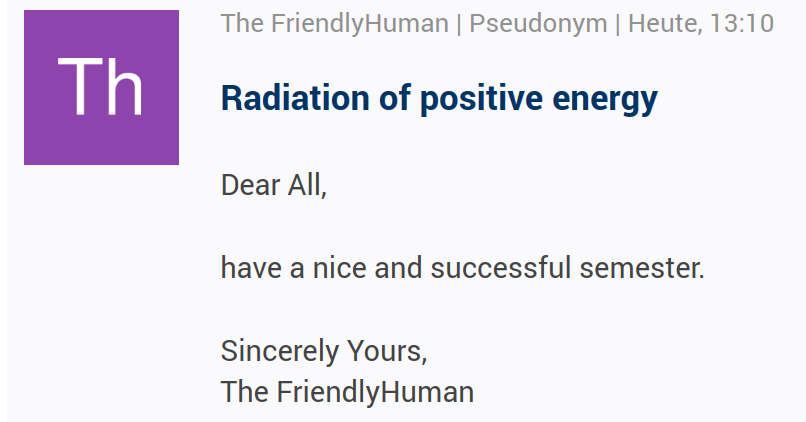
\includegraphics[width=0.7\textwidth]{images/positive_energy.png}%
        %
    \end{figure}
\end{frame}

